% -*- TeX-master: "../dipole_ilya_paper.tex" -*-
\section{Operations with qubits}
\label{sec:characterisation}

\red{Need scattering data}

\red{Coupling data and comparison of dipole moments between RF and twin qubits}

\noindent We measure transmission of microwave signals at different frequencies when the qubit
is  biased by  an  external magnetic  flux  close  to the  degeneracy  point $  \frac{1}{2}\Phi_0
$. Because of a  small asymmetry, $\eta$, the fluxes linked through the  left and right loops are
different, $ \Phi = \frac{\varphi}{2\pi}\Phi_0$ and $ \eta\Phi $.

The \iket{1}~\ilra~\iket{2} transition, $\omega_{21}$, is seen as a suppression of transmission, in
accordance  with the  scattering \cite{Astafiev2010}.   a Vector  Network Analyzer  (VNA) that
sends in  a microwave signal  of a particular  frequency, $\omega_{\text{VNA}}$, and  monitors it's
amplitude  after   it  has   passed  through   the  system.   As   shown  in   previous  works
\cite{abdumalikov2010},   the    transmission   amplitude    is   suppressed    at   resonance
($\omega_{\text{VNA}}=\omega_{21}$).   This resonance  condition  is  mapped out  with  blue circles  in
Fig.~\ref{fig:experiment}.   The resonance  is  period  in flux,  with  a  tendency of  higher
$\omega_{21}$  at  higher  magnetic  flux numbers.   \red{Explain  resonant  emission,  destructive
  interference and show graph the transmission dip}

The \iket{2}\ilra\iket{3}  transition, $\omega_{32}$,  is mapped  using two-tone  spectroscopy: the
network  analyzer is  tuned  to the  transition  frequency  $ \omega_{21}  $,  while an  additional
microwave generator  sweeps a  second frequency,  $ \omega_{\text{GEN}}  $. Whenever  the generator
strikes the  \iket{2}\ira\iket{3} transition ($\omega_{\text{GEN}} =  \omega_{32} $), the qubit  will be
excited  in  a  sequence   \iket{1}  \iratext{$\omega_{21}$}\iket{2}  \iratext{$\omega_{32}$}  \iket{3},
depopulating state \iket{1}.  This  will show up in an improved transmission  of the signal at
$\omega_{21}$,   as  state   \iket{1}   depopulates   completely  to   the   higher  levels.    The
$\omega_{32}$ transition is mapped with red circles in Fig.~\ref{fig:experiment}. \red{parameters?}

% prove that state 1 becomes depopulated by solving the master equation for two drives

\begin{figure}[h]
  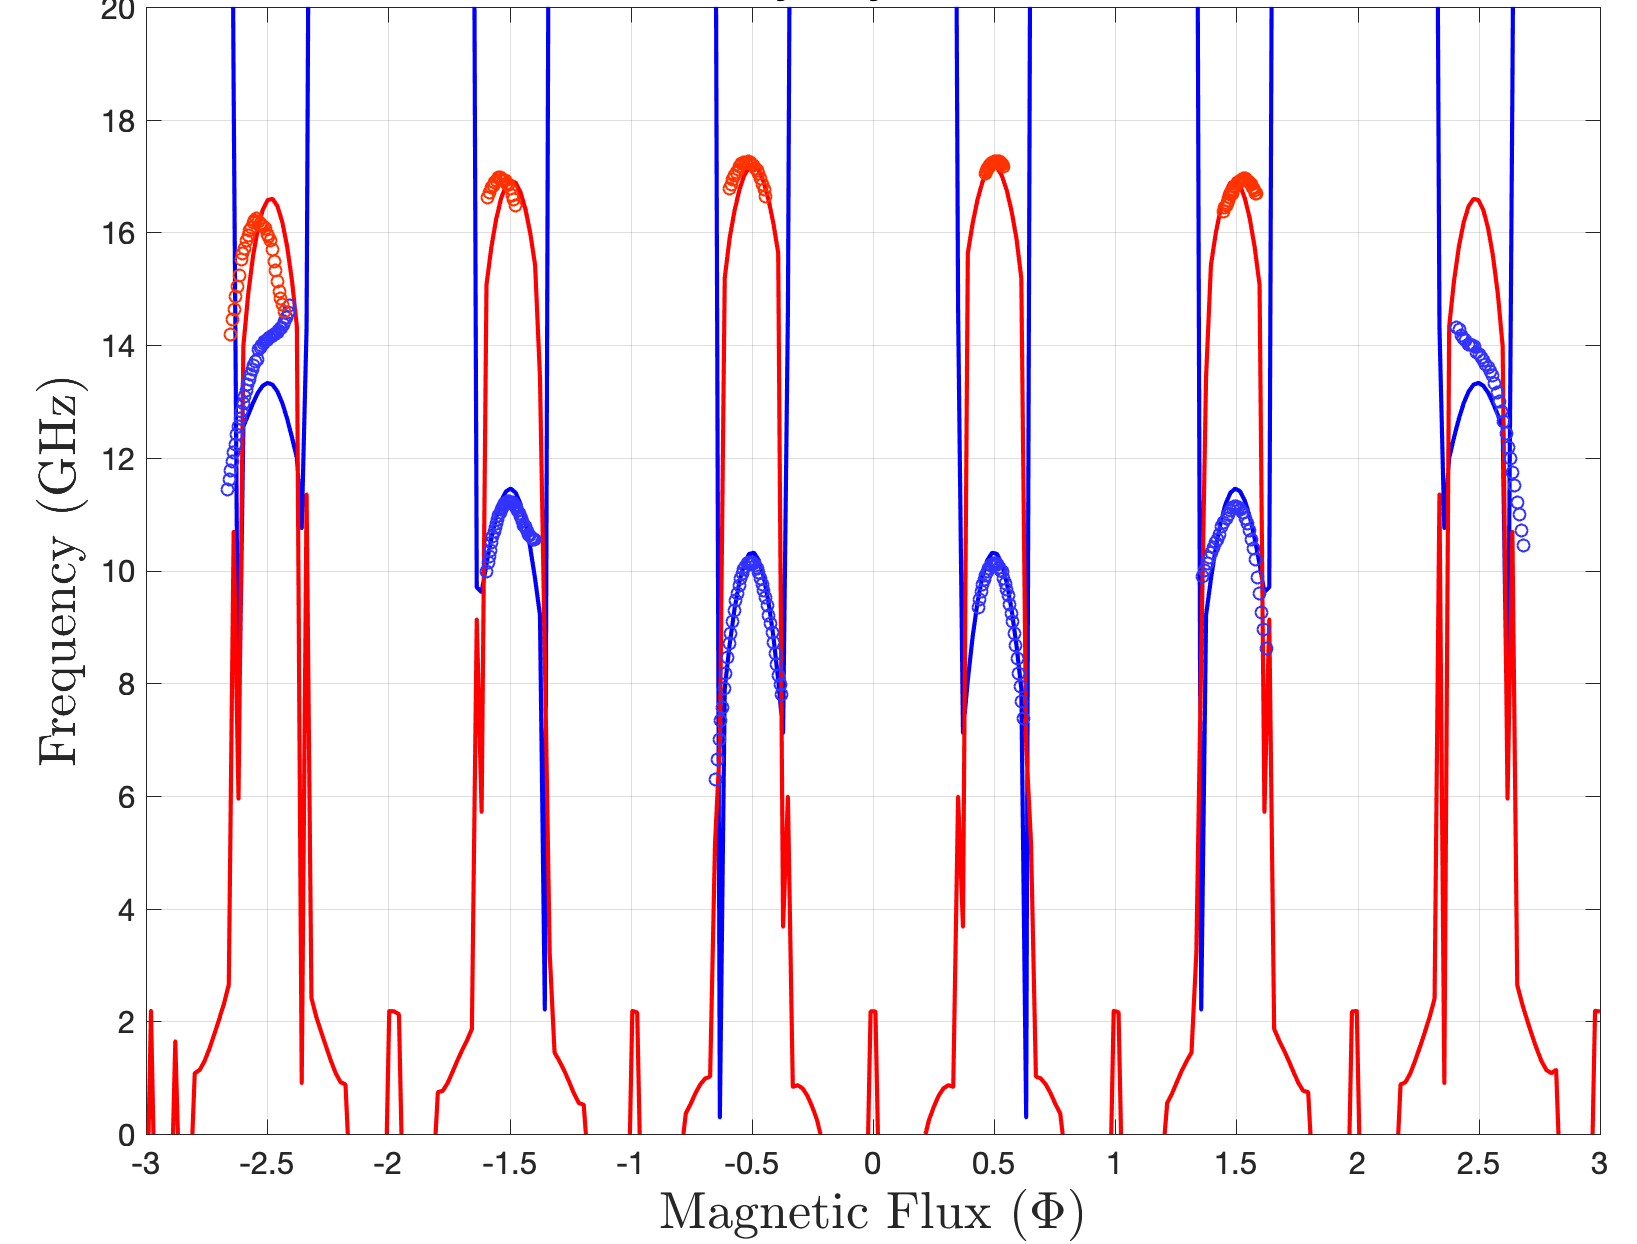
\includegraphics[height=6cm]{figure3_qubit2}
  \caption{\small    Transition   frequencies    between   levels    \iket{1}\ilra   \iket{2},
    $  \omega_{21}  $  (blue),  and  \iket{2}  \ilra  \iket{3},  $  \omega_{32}$  (red).   Readings  for
    $    \omega_{32}    $     are    in    a    narrow    flux    range     because    away    from
    $  \Phi  =  (n +  \frac{1}{2})\Phi_0,  n\in\mathbb{Z}  $,  it  gets  harder  to tune  the  VNA  to
    $ \omega_{21} $  (as part of the  two-tone spectroscopy procedure) which  prevents the accurate
    mapping of $  \omega_{32} $ with the second  tone.  Asymmetry in the flux  penetrating the left
    and  right loops  results  in the  gradual  change of  transition  frequencies with  every
    $ \Phi_{0}  $ period -  $\omega_{21}$ creeps  up, while $\omega_{32}$  creeps down, breaking  the usual
    periodicity in flux qubits.}
  \label{fig:experiment}
\end{figure}

We  match the  experimental  data points  to  simulations made  on  the system's  Hamiltonian,
$ \mathcal{H}  = T + U  $, developed using  the standard approach for  quantum electrodynamics
\cite{orlando1999}. Islands,  isolated by the JJ  in Fig.~\ref{fig:setup}, are labeled  with a
Cooper    pair     occupation    $     \vec{n}    =    (n_1,     n_2,    n_3)     $,    phases
$        \vec{\varphi}       =        (\varphi_1,        \varphi_2,       \varphi_3)        $       and        voltage
$ \vec{V} = \left(V_{1}, V_{2}, V_{3}\right) $.   An inspection of the system's topology links
the sets

\begin{equation}
  \label{eq:link}
  2e\vec{n} = \hat{C}\vec{V}
\end{equation}

\noindent through the capacitance matrix

\begin{equation}
  \label{eq:capac}
  C = \iabs{C} \begin{pmatrix}
    2  &  -1  &  0\\
    -1  &  2  +  \alpha  &  -1\\
    0  &  -1  & 2
  \end{pmatrix}
\end{equation}

\noindent  where \iabs{C}  is the  capacitance of  the outer  JJs. The  total charging  energy
resulting from the interaction between charge of  the Cooper pairs, $ \vec{Q}=2e\vec{n} $, and
voltages on the islands gives rise to the kinetic term of the Hamiltonian:

\begin{equation}\label{eq:kinetic}
  \begin{aligned}
    T & = \frac{1}{2}\sum_{i=1}^{3}Q_iV_i = \frac{(2e)^2}{2}\vec{n}\hat{C}^{-1}\vec{n}^{T}.
  \end{aligned}
\end{equation}

Each of the 5 JJs each contribute $  E_{Ji}\left(1 - \cos(\varphi_i)\right) $ to the potential term.
The  two junction  phases unspecified  by $  \vec{\varphi}  $ are  pinned by  the flux  quantization
condition          for          the           left          and          right          loops,
$  \sum_i^{\text{loop}}  \varphi_i =  2\pi  n,  n \in  \mathbb{Z}}$,  which  have external  biasing  fluxes
$ \varphi_\text{ext} $, $ \eta\varphi_\text{ext} $:
\begin{equation}\label{eq:potential}
  \begin{aligned}
    U & = E_J\big[4 + \alpha - \alpha\cos(\varphi_{2}) -\cos(\varphi_{1}) -\cos(\varphi_{3}) - \\
    & \qquad \cos(\varphi_{2} - \varphi_{1} - \varphi_{\text{ext}}) - \cos(\varphi_{2} - \varphi_{3} + \eta\varphi_{\text{ext}})\big].
  \end{aligned}
\end{equation}

The Hamiltonian matrix  is encoded in the Cooper  pair number basis, $\vec{n} $,  in which the
kinetic terms are on the diagonal and the potential terms are distributed symmetrically on the
off  diagonal  positions.   The  phase  operators in  the  number  basis  representation  read
$ e^{\pm i\hat{\varphi}_j} = \sum_{n_i}\iketbra{n_i\pm1}{n_i}$  \cite{phase}.  The eigenenergies of the
resulting Hamiltonian  are compared  with the  experimental data  in Fig.~\ref{fig:experiment}
using  \iunit{E_J =  91.0}{GHz}, \iunit{E_C  = 13.50}{GHz},  \iunit{\alpha =  1.023}{}, \iunit{\eta  =
  1.011}{}.  The asymmetry value, $ \eta $, is  close the visual loop area difference of 3\% seen
from the SEM image in Fig.~\ref{fig:setup}.
 
 \begin{figure}[h!]
   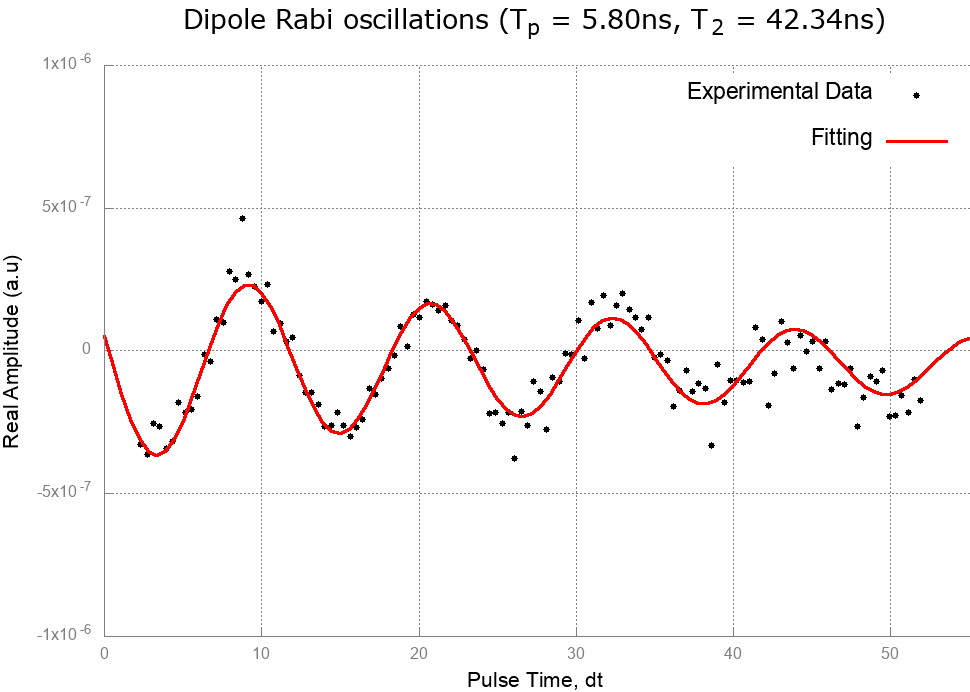
\includegraphics[height = 5cm]{figure5}
   \caption{Rabi oscillation taken  at the degeneracy point,  $ \Phi_0/2 $, by  driving the qubit
     with  resonant  microwaves,  $\omega_{\text{VNA}}  =   \omega_{21}$  for  different  time  periods,
     $ dt $, and monitoring the signal in  the output line \cite{rabi}. The a decoherence time
     of  $  \tau_{\text{dec}}   =  \iunit{42}{ns}  $  is  extracted  from   the  decay  envelope,
     $ e^{-dt/\tau_\varphi} $, of the the oscillations. \label{fig:rabi}}
 \end{figure}

 An important qubit parameter  is the curvature at the turning points  in the energy spectrum,
 where qubit operations are carried out. A low  curvature is desirable, to make the qubit less
 sensitive  to external  flux changes,  which  would improve  decoherence time.   At the  twin
 qubits'  degeneracy point  $ \Phi  =  (n +  \frac{1}{2})\Phi_0,  n\in\mathbb{Z} $,  the curvature  is
 $   -550\pm10\,\text{GHz}/\Phi_0^2  $.    It  is   substantially  smaller   than  $   13\times  10^4$
 $ \text{GHz}/\Phi_0^2$ on the 4-JJ flux qubit \cite{stern2014}, $ 8.4 \times 10^4$ \cite{zhu2010} and
 $ 37\times 10^{4}$ $ \text{GHz}/\Phi_0^2$ \cite{gustavsson2012}  on the 3-JJ flux qubits demonstrated
 recently.   The  decoherence   time  in  our  qubits  was  however   relatively  small,  only
 $  \tau_\text{dec}  =  \iunit{42}{ns}  $.   We   get  $\tau_\text{dc}$  from  measurement  of  Rabi
 oscillations,  see Fig.~\ref{fig:rabi}  \cite{rabi}.  We  explain  this by  poisoning of  the
 sample  with  infrared radiation,  and  simplified  technology  used  for fabrication  as  we
 mentioned above.

 Despite the twin  qubit have a much the  decoherence time in our qubits  was relatively small
 This improved robustness to  flux noise is matched by a decoherence time  of , extracted from
 Rabi oscillations in Fig.~\ref{fig:rabi} \cite{rabi}.

%%% Local Variables:
%%% mode: latex
%%% TeX-master: "../dipole_ilya_paper"
%%% End:
